\section{Two particles in one chamber}\label{sec:twoparticle}
\sectionstate{partial}{\texttt{rerun/effbudget/single} (\texttt{single\_track\_area.py}, \texttt{xy\_pairing.py},
\texttt{PAIRING\_FIX\_2026-11-02.md}, \texttt{MERGED\_PROJECTION\_2026-11-02.md}); figure \texttt{papers/paper1\_v2/figs/make\_pairing.py},
numbers \texttt{figs/out/pairing.json}, bookkeeping \texttt{figs/out/two\_particle\_numbers.md}; charge balance
\texttt{rerun/paper1\_charge}. v2 2026-11-10: the old sections 5.1 and 5.5, results only; how the reconstruction got there
(the joint fit, the veto rescue) is in \cref{app:moved}.}
\intent{The result specific to this readout: both views see the same charge, and that is what tells which X segment
belongs to which Y segment when two particles cross one chamber.}

A chamber with two strip views has no direct way to tell which segment in X belongs to which segment in Y. With one
particle there is nothing to tell. With two there are two ways to pair the segments, and the wrong one makes two
ghost tracks. The views share no coordinate, but in this design they share something else: every avalanche lands on
pads that alternate between the X and the Y strips, so both views read the same charge at the same time.

\subsection{The two views see the same charge}\label{sec:balance}
\Crefp{fig:pairing}{a} shows the balance for single tracks. The fraction of the charge read by the X strips,
$f=q_X/(q_X+q_Y)$, has a median of 0.485 in chamber~A and 0.513 in chamber~B, and between 0.485 and 0.509 in the
others. Track by track the ratio $q_X/q_Y$ of chamber~A scatters by 6\,\% (a core spread of 0.014 in $f$; 0.017 to
0.028 in the other chambers), and the balance does not depend on position or angle. Chamber~D has the same core, but a
quarter of its tracks lie in a tail, from the fault of its X readout.

\subsection{Finding the muon when it is not alone}\label{sec:twoeff}
In 3.2\,\% of the events (931 of 29\,398) a second particle crosses chamber~A with the muon. These are the events in
which a second segment appears in both views with matching charge, in one of three configurations
(\cref{fig:twoparticle}):
\begin{itemize}
  \item the two particles are separate in both views (662 events): the muon is detected in $95.6\pm0.8$\,\%, as often
  as when it is alone;
  \item they are separate in one view and merged in the projection of the other (176 events): $47\pm4$\,\%;
  \item the muon is clean in both views and a separate, large deposit lies elsewhere in the plane, so that the event
  exceeds the 50 strips at which the reconstruction treats it as a discharge and fits nothing (93 events): 1\,\%.
\end{itemize}
Over all of them the muon is detected in $77.0\pm1.4$\,\%. The reconstruction addresses the second configuration with
a joint fit that offers a merged column a second track when the charge of the other view corroborates it. On a fixed
set of 195 merged events this raises the detection of the muon from 41 to 54\,\% without splitting a clean single muon
in any of the five chambers; what remains unsplit are pairs that share almost no depth or lie within four strip
pitches of each other.
\askDylan{The third configuration is a loss of the discharge veto, not of two-track reconstruction; its display moved to
the gallery of \cref{app:effdef}. The counts 146, 195, 232 and 176 for ``merged events'' in the old text belong to three
classifiers and two versions of the reconstruction; only 176 (final reconstruction, full area) and the 195-event validation set
are used here.}

\begin{figure}[tbp]
  \centering
  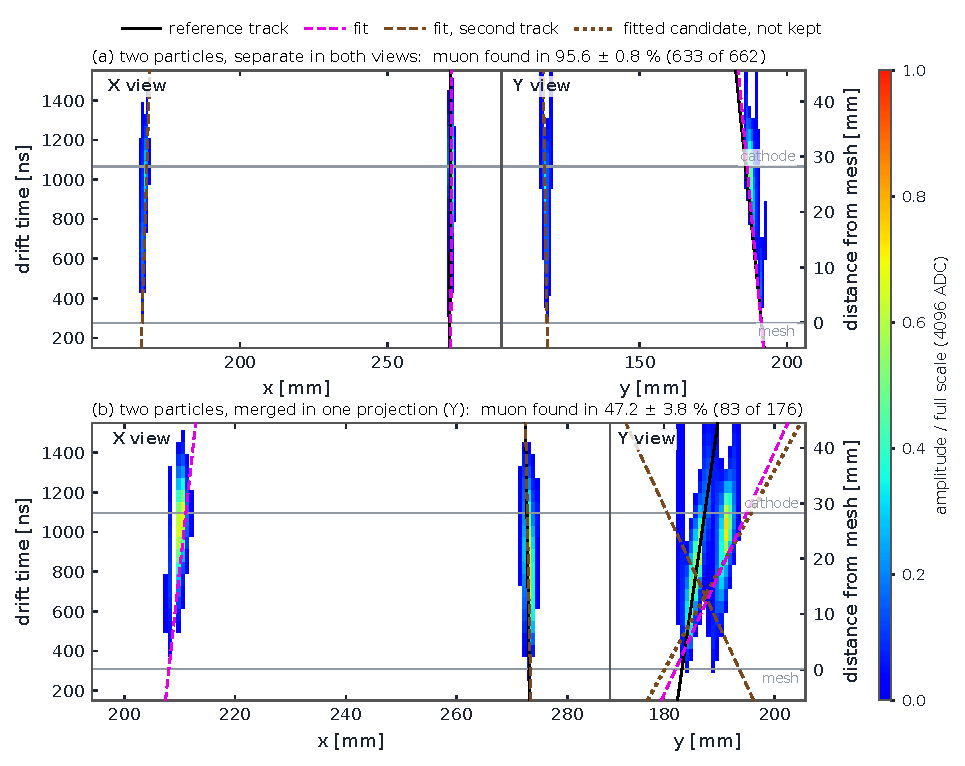
\includegraphics[width=0.9\linewidth]{two_particle_ab}
  \caption{Two particles in chamber~A, one real event per configuration (Run~1; both views, strip position against
  drift time, amplitude normalised to the full scale of the ADC; reference track solid black; fits dashed, magenta the
  first track and brown the second, dotted a fitted candidate that was not kept; grey lines, mesh and cathode). Each
  title gives the fraction of such events in which the muon is reconstructed within 5\,mm of the reference. (a)
  Separate in both views: both are fitted, and the muon is found as often as alone. (b) Two columns 63\,mm apart in X,
  merged into one broad column in Y: the joint fit splits the Y column in two. The track within 5\,mm of the reference
  counts as the muon, but here it is paired with the other particle's X segment, and its angle differs from the
  reference's.}
  \label{fig:twoparticle}
\end{figure}

\subsection{Pairing the views}\label{sec:pairing}
The test of pairing uses 567 two-particle events in which the reference track marks one of the two particles in both
views, so that the right pairing is known. \Crefp{fig:pairing}{b} shows the charge ratio of the right and of the
swapped pairing in these events: the right one sits on the single-track balance, the swapped one is spread over a
factor of several. Choosing the pairing whose charge ratios are closer to the single-track value is right in
95.6\,\% of the events.

The drift gives a second handle. The charge of one particle arrives at the same times in both views, and that of
two particles at different depths does not: the median arrival times of a right pair agree to 48\,ns, those of a
swapped pair to 176\,ns (\crefp{fig:pairing}{d}). With charge and time together the pairing is right in
\[ 97.7\pm0.6\ \%.\]
The failures are where they should be (\crefp{fig:pairing}{c}): every event in which the two particles differ in charge
by more than a factor 1.65 is paired correctly (290 of 290), and all failures have particles of nearly equal charge.
The reconstruction makes the same choice by a cost that adds further timing terms, and on the same 567 events it
pairs $96.6\pm0.8$\,\% correctly~\cite{paperII}.
\askDylan{The old text also listed ``A 95.9, B 96.8, C 92.2, D 90.1, E 94.0\,\%'' for the production pairing. That is another
sample (all runs of each chamber, first-version tables with the pairing selection replayed), which is why A read 95.9 there and
96.6 here. It could go in the summary table as ``pairing, all runs'' if you want the other chambers shown.}

This is the feasibility demonstration for pairs: with a single plane of pads read in two views, a chamber separates
and pairs two tracks without a third coordinate.

\begin{figure}[tbp]
  \centering
  \figorbox[width=0.9\linewidth]{pairing}{charge balance, true and swapped pairings, pairing fraction against charge ratio, arrival-time difference}
  \caption{Pairing the X and Y views when two particles cross chamber~A. (a) The X/Y charge balance $\ln(q_X/q_Y)$
  of 24\,510 single tracks (Runs 1 and 2); inset: median and core spread per chamber (long runs, unsaturated tracks).
  (b) $\ln(q_X/q_Y)$ of the true (reference-tagged) and the swapped pairings in 567 two-particle events; grey, the
  single-track $\pm1\sigma$ band. (c) Fraction of events paired correctly against the ratio of the charges of the two
  particles, using the charge balance alone (open) and the charge balance with the arrival-time difference (filled);
  68\,\% binomial intervals, the number of events per bin below the points. (d) Difference between the views of the
  median charge-arrival time for the true and the swapped pairings; grey, the single-track band.}
  \label{fig:pairing}
\end{figure}

\subsection{How close two tracks can be}\label{sec:separation}
Real two-particle events cannot say how close two tracks may come before they are no longer resolved: the second
particle has no reference, and the separation is unknown exactly where the tracks merge. The measurement is made by
overlay instead. The waveforms of two real single-muon events of chamber~A are added, with their own positions, and
the sum is passed through the same reconstruction; each muon keeps its own reference track.
\tbw{Result: the probability that both muons are reconstructed against their separation in the closer view
(\crefp{fig:separation}{a}), and the resolution of the opening angle of the pair (\crefp{fig:separation}{b}).}
\analysis{SEP}{not yet run on the final reconstruction. The overlay script and a batch job are written and tested
(\texttt{papers/paper1\_v2/figs/make\_two\_track\_separation.py}, \texttt{figs/two\_track\_batch/README.md}): 2\,400 overlays,
about 6 core-hours, which is over the limit for the laptop, and submitting needs a login on lxplus. A test of 8 overlays
per bin ran end to end: an overlay with an empty partner returns the single-track result (8 of 8 found, 0.91\textdegree{}
X), both muons were reconstructed in every overlay above 18\,mm, and the opening angle of resolved pairs came out near
1.5\textdegree{} in space; with 8 events per bin none of this is quotable. On an earlier reconstruction (26 October) the
standard chain resolved nothing below 12\,mm, the joint fit 28/43/50\,\% at 0--6/6--12/12--18\,mm, and the opening angle
was measured to 1.47\textdegree{} above 24\,mm. Caveats to state with the result: both particles are minimum-ionising muons
within $\pm20$\textdegree, the noise is added twice, the sum saturates at the ADC limit of the first event, and the two
events have independent triggers.}
\begin{figure}[tbp]
  \centering
  \figorbox{two_track_separation}{probability of resolving both tracks against their separation; resolution of the opening angle}
  \caption{\tbw{Two-track performance of chamber~A from overlays of two single-muon events. (a) Probability that both
  muons are reconstructed, against their separation at mid-gap in the closer view. (b) Resolution of the opening angle
  of the pair. (c) Error on the reconstructed separation.}}
  \label{fig:separation}
\end{figure}
